\documentclass[border=4pt]{standalone}
\usepackage{amsmath}
\usepackage[T1]{fontenc}
\usepackage{newtxtext,newtxmath}
\usepackage{tikz}
\usetikzlibrary{arrows.meta,positioning,fit,calc}
\begin{document}
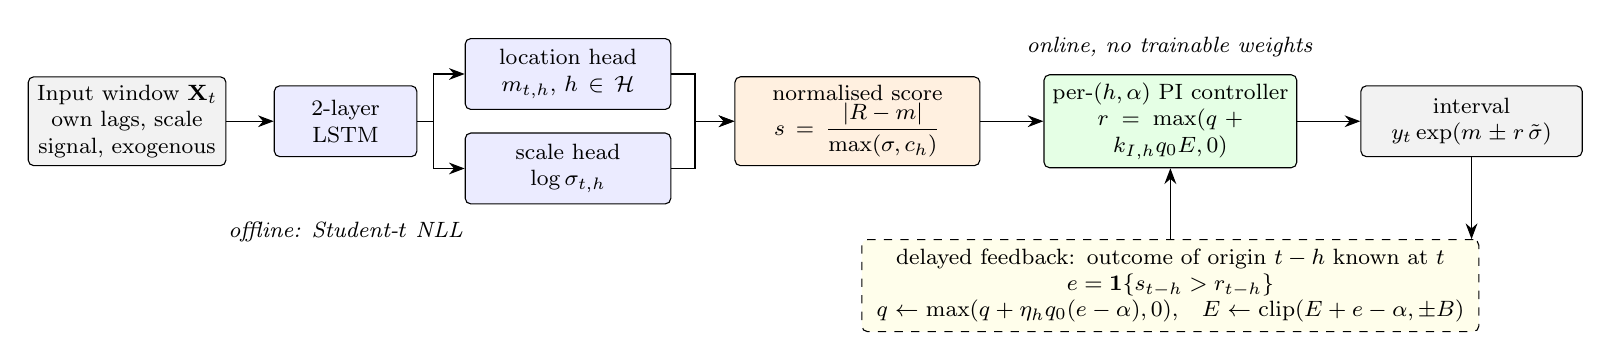
\begin{tikzpicture}[
  font=\footnotesize, >={Stealth[length=2mm]},
  box/.style={draw, rounded corners=2pt, align=center, minimum height=9mm, inner sep=3pt, fill=#1},
  box/.default=white]
  \node[box=gray!10, text width=2.3cm] (in) {Input window $\mathbf{X}_t$\\ own lags, scale\\ signal, exogenous};
  \node[box=blue!8, right=6mm of in, text width=1.6cm] (lstm) {2-layer\\ LSTM};
  \node[box=blue!8, right=6mm of lstm, text width=2.4cm, yshift=6mm] (mu) {location head\\ $m_{t,h}$, $h\in\mathcal{H}$};
  \node[box=blue!8, right=6mm of lstm, text width=2.4cm, yshift=-6mm] (sg) {scale head\\ $\log\sigma_{t,h}$};
  \node[box=orange!12, right=8mm of mu, text width=2.9cm, yshift=-6mm] (sc) {normalised score\\ $s=\dfrac{|R-m|}{\max(\sigma,c_h)}$};
  \node[box=green!10, right=8mm of sc, text width=3.0cm] (pi) {per-$(h,\alpha)$ PI controller\\ $r=\max(q+k_{I,h}q_0E,0)$};
  \node[box=gray!10, right=8mm of pi, text width=2.6cm] (out) {interval\\ $y_t\exp(m\pm r\,\tilde\sigma)$};
  \draw[->] (in) -- (lstm);
  \draw[->] (lstm.east) -- ++(2mm,0) |- (mu.west);
  \draw[->] (lstm.east) -- ++(2mm,0) |- (sg.west);
  \draw[->] (mu.east) -- ++(3mm,0) |- (sc.west);
  \draw[->] (sg.east) -- ++(3mm,0) |- (sc.west);
  \draw[->] (sc) -- (pi);
  \draw[->] (pi) -- (out);
  \node[draw, dashed, rounded corners=2pt, below=9mm of pi, text width=7.6cm, align=center, fill=yellow!8] (fb)
     {\mbox{delayed feedback: outcome of origin $t-h$ known at $t$}\\
      \mbox{$e=\mathbf{1}\{s_{t-h}>r_{t-h}\}$}\\
      $q\leftarrow\max(q+\eta_h q_0(e-\alpha),0)$,\quad
      $E\leftarrow\mathrm{clip}(E+e-\alpha,\pm B)$};
  \draw[->] (out.south) -- (out.south |- fb.north);
  \draw[->] (fb.north) -- (pi.south);
  \node[below=7mm of lstm, align=center] {\textit{offline: Student-$t$ NLL}};
  \node[above=1mm of pi, align=center] {\textit{online, no trainable weights}};
\end{tikzpicture}
\end{document}
